%---------- Primeiro Capitulo ----------
\chapter{Introdução}\label{cha:introducao}

A evolução tecnológica, presente nos dias de hoje, possibilitou o desenvolvimento de dispositivos móveis que não são mais usados somente para a comunicação, mas para a execução de diversas aplicações que oferecem funcionalidades com alta qualidade de serviço, para as quais, há alguns anos atrás seriam necessários diversos equipamentos dedicados, como no exemplo da Figura \ref{fig:convergencia} onde podemos perceber a convergência de algumas funcionalidades desses aparelhos para os dispositivos móveis: um aparelho de som, aparelho dedicado para o uso de \sigla{GPS}{Global Positioning System} (\textit{Global Positioning System}), câmera de alta resolução para tirar fotos e realizar a gravação de áudio e vídeo, computador para a comunicação através de redes \sigla{Wi-Fi}{Wireless Fidelity} (\textit{Wireless Fidelity}) e também o uso de \textit{video-games}.

\begin{figure}[!htb]
	\centering
	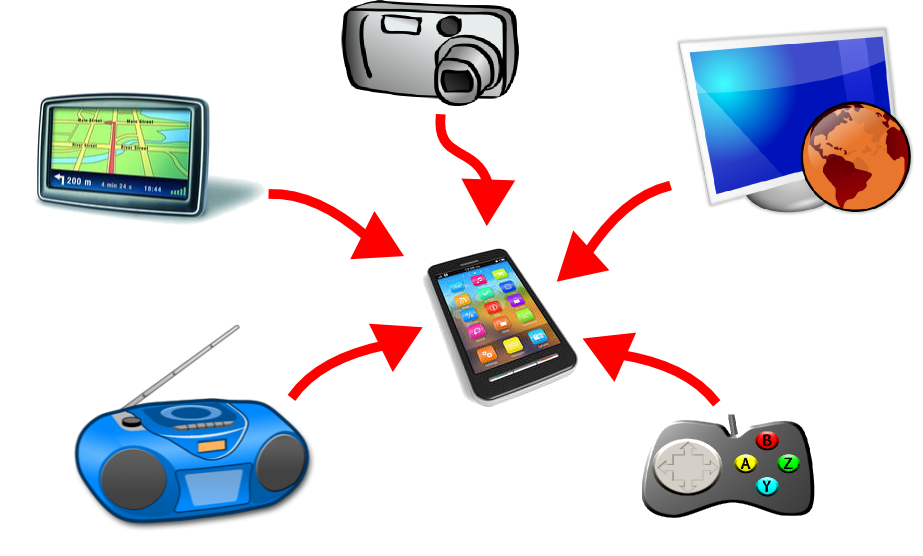
\includegraphics[width=0.5\textwidth]{convergencia.png} % <- formatos PNG, JPG e PDF
	\small
	\caption[Convergência de diversos equipamentos para um dispositivo móvel]{Convergência de diversos equipamentos para um dispositivo móvel}
	\label{fig:convergencia}
\end{figure}

Com o uso das redes sem fios, que disponibilizam o uso da Internet nos dispositivos móveis, a quantidade de serviços e conteúdos oferecidos aos usuários é imensa. Podem ser utilizados serviços como: correio eletrônico, navegação em sites, troca de mensagens instantâneas, download e upload de arquivos, conexão a bancos de dados, o uso de streaming de áudio e vídeo, e tudo o mais que a Internet possa oferecer.

Todos esses serviços e produtos que estão disponíveis na Internet se beneficiam da qualidade das redes de computadores, como por exemplo, uma boa largura de banda e equipamentos de última geração, mas também podem ser prejudicados por alguma deficiência ou problema que aconteça com a rede, como o defeito em algum roteador, o congestionamento na rede ou uma arquitetura mal dimensionada. Assim, cada um dos provedores de conteúdo que o usuário acessa pode apresentar atributos relacionados aos serviços oferecidos, como por exemplo: número de clientes conectados, tempo de resposta, custo da licença para usar o serviço e a qualidade do serviço prestada.

Os valores desses atributos podem ser modificados dependendo do contexto em que se encontra esse provedor. Dessa forma, esse conjunto de atributos pode ser relevante para o usuário no momento da escolha do provedor de conteúdo que atenderá as suas expectativas de forma satisfatória. Como essas informações podem ser alteradas, um serviço escolhido poderá não mais atender ao usuário de forma satisfatória, assim ele poderá procurar outro serviço semelhante que lhe atenda da forma desejada. Neste trabalho, essas informações são importantes para que seja feita a escolha do provedor de serviço de forma automatizada, elas determinam qual é o provedor que o usuário escolheria.

Este trabalho tem como base o trabalho realizado na dissertação de mestrado em Ciência da Computação de \cite{praca12}, onde foi descrito um modelo de autenticação baseado em informações de contexto, denominado HandProv, no qual o usuário efetua handover (troca de conexão de um ponto de acesso para outro sem perda ou interrupção dos serviços) de provedores de serviço de forma transparente. As trocas de provedores aconteciam baseando-se nos valores de alguns atributos, onde o gerente de aplicações escolhia o provedor que melhor atendesse ao usuário. 

\section{Motivação}
O grande salto na quantidade de dispositivos móveis utilizados pela população em geral, fez com que aparecessem novas necessidades de software. Alguns desses sistemas têm como objetivo a facilitação de resolução de tarefas do cotidiano do usuário.
A disseminação do uso das redes sem fio, Wi-Fi e 3G, que possibilitam aos usuários estarem conectados à Internet, com uma boa largura de banda, faz com que os usuários passem uma parte considerável de seu tempo utilizando serviços e recursos disponibilizados pela rede.
Devido a essa grande quantidade de serviços disponíveis e muitos deles oferecendo o mesmo tipo de conteúdo o usuário tem a opção de escolher o que atenda-o da melhor maneira.

\section{Objetivos e Contribuições}
Este trabalho teve como objetivo a implementação de duas aplicações, uma aplicação para dispositivos móveis onde o usuário configura os seus requisitos para cada provedor de serviço e que também apresenta os serviços ao usuário e uma aplicação servidora que realiza a escolha de qual serviço atende aos requisitos do usuário e que realiza as autenticações necessárias nos serviços de forma transparente.

Através dos estudos realizados sobre as tecnologias utilizadas e das implementações dos sistemas, este trabalho ficará disponível à comunidade acadêmica como um exemplo de uma aplicação desenvolvida para dispositivos móveis que utiliza novas tecnologias, como por exemplo um banco de dados NoSQL\footnote{Sistemas de bancos de dados que utilizam formas de armazenar e devolver dados diferente dos que utilizam tabelas relacionais} e o desenvolvimento utilizando ferramentas disponibilizadas na nuvem.

A contribuição que este trabalho faz em relação ao trabalho de \cite{praca12} é a apresentação de um modelo onde são os provedores de serviço que determinam quais são seus atributos e o usuário apenas configura os valores que ele considera relevantes a ele, e a implementação de uma estrutura na aplicação do dispositivo móvel que permite a renderização de formulários dinâmicos, que pode sofrer alterações no seu desenho de acordo com as alterações dos atributos dos provedores sem a necessidade de alterações no código fonte da aplicação.

\section{Organização do trabalho}
Neste trabalho o termo 'Dispositivos Móveis' será utilizado para representar o termo em inglês Smartphones, que categoriza uma linha de aparelhos celulares com sistemas operacionais multitarefas.

Este trabalho está organizado da seguinte maneira. O Capítulo \ref{cha:introducao} apresenta o cenário no qual o trabalho se encaixa, a motivação e os objetivos desse trabalho. O Capítulo \ref{cha:fundamentacao} apresenta os principais conceitos sobre autenticação em sistemas computacionais. O Capítulo \ref{cha:visaogeral} apresenta algumas das principais tecnologias sobre dispositivos móveis presentes no mercado atualmente. O Capítulo \ref{cha:ferramentas} apresenta algumas das tecnologias mais conhecidas para o desenvolvimento de aplicativos móveis. O Capítulo \ref{cha:desenvolvimento} apresenta os sistemas que foram implementados e como eles funcionam. O Capítulo \ref{cha:conclusao} finaliza o trabalho de conclusão de curso com as contribuições e trabalhos futuros.